% 5-minute thesis presentation
% Compile with: lualatex thesis_5min_presentation.tex
\documentclass[aspectratio=169,12pt]{beamer}

% ---------- Fonts ----------
\usepackage{fontspec}
\defaultfontfeatures{Ligatures=TeX}
\IfFontExistsTF{Roboto}{%
  \setsansfont{Roboto}[
    UprightFont = * Light,
    BoldFont = * Medium,
    ItalicFont = * Light Italic,
    BoldItalicFont = * Medium Italic
  ]
}{%
  \setsansfont{Arial}
}
\renewcommand{\familydefault}{\sfdefault}
\usefonttheme{professionalfonts}

% ---------- Packages ----------
\usepackage{amsmath,amssymb,mathtools}
\usepackage{tikz}
\usetikzlibrary{arrows.meta,positioning,calc,decorations.pathreplacing,fit,backgrounds,shapes.geometric,shapes.misc}
\usepackage{pgfplots}
\pgfplotsset{compat=1.18}
\usepackage{booktabs,array,colortbl,tabularx}
\usepackage{ragged2e}
\usepackage{graphicx}
\usepackage{bbm}
\usepackage{hyperref}
\usepackage{comment}
% If not already in your preamble: % 
\usetikzlibrary{arrows.meta} 
% Softer pipeline colors, closer to the generated image 
\definecolor{PipeBlue}{HTML}{1F78B4} 
\definecolor{PipeGreen}{HTML}{3F8F3B} 
\definecolor{PipeGold}{HTML}{B8870A} 
\definecolor{PipePurple}{HTML}{7B4D7D} 
\definecolor{PipeTeal}{HTML}{168A8A}

% ---------- Colors ----------
\definecolor{PrimerNavy}{HTML}{012169}
\definecolor{PrimerText}{HTML}{333333}
\definecolor{PrimerMuted}{HTML}{777777}
\definecolor{PrimerLight}{HTML}{EFEFEF}
\definecolor{PrimerRule}{HTML}{D9D9D9}
\definecolor{PrimerRed}{HTML}{B75C4C}
\definecolor{PrimerTeal}{HTML}{0C7893}
\definecolor{PrimerOrange}{HTML}{D55E00}
\definecolor{PrimerBlue}{HTML}{0072B2}
\definecolor{PrimerGreen}{HTML}{1B9E77}

% ---------- Beamer reset ----------
\setbeamercolor{background canvas}{bg=white}
\setbeamercolor{normal text}{fg=PrimerText,bg=white}
\setbeamercolor{frametitle}{fg=PrimerText,bg=white}
\setbeamercolor{page number in head/foot}{fg=PrimerMuted}
\setbeamercolor{structure}{fg=PrimerTeal}
\setbeamertemplate{navigation symbols}{}
\setbeamertemplate{headline}{}
\setbeamersize{text margin left=0.74cm,text margin right=0.74cm}

\setbeamerfont{normal text}{size=\fontsize{9.4}{13.5}\selectfont}
\setbeamerfont{frametitle}{size=\fontsize{16.0}{20}\selectfont,series=\mdseries}
\setbeamerfont{title}{size=\fontsize{16.0}{20}\selectfont,series=\mdseries}
\setbeamerfont{subtitle}{size=\fontsize{9.8}{12}\selectfont,series=\mdseries,shape=\itshape}
\setbeamerfont{author}{size=\fontsize{7.2}{9}\selectfont,series=\bfseries}
\setbeamerfont{institute}{size=\fontsize{7.2}{9}\selectfont,shape=\itshape}
\setbeamerfont{caption}{size=\fontsize{7.2}{9}\selectfont}

\setbeamertemplate{frametitle}{%
  \vspace*{0.42cm}%
  \hspace*{-0.02cm}\insertframetitle\par%
  \vspace*{0.20cm}%
}

\setbeamertemplate{footline}{%
  \begin{beamercolorbox}[wd=\paperwidth,ht=0pt,dp=0pt]{page number in head/foot}%
  \begin{tikzpicture}[remember picture,overlay]
    \node[anchor=south east, font=\fontsize{4.8}{6}\selectfont]
      at ([xshift=-0.50cm,yshift=0.22cm]current page.south east)
      {\insertframenumber{} / \inserttotalframenumber};
  \end{tikzpicture}%
  \end{beamercolorbox}%
}

% ---------- Useful macros ----------
\newcommand{\red}[1]{\textcolor{PrimerRed}{#1}}
\newcommand{\teal}[1]{\textcolor{PrimerTeal}{#1}}
\newcommand{\muted}[1]{\textcolor{PrimerMuted}{#1}}
\newcommand{\pstrong}[1]{{\bfseries #1}}
\newcommand{\arrowtext}[1]{\par\vspace{0.45em}\noindent{\fontsize{10}{12}\selectfont $\to$}\hspace{0.45em}{#1}\par}
\newcommand{\spacedparagraph}[1]{\par\noindent\begin{minipage}{0.96\linewidth}\RaggedRight #1\end{minipage}\par\vspace{0.55em}}
\newcommand{\smallref}[1]{\vspace{0.15cm}{\fontsize{5.8}{7}\selectfont\muted{#1}}}

\newcommand{\sectionframe}[1]{%
{%
\setbeamercolor{background canvas}{bg=PrimerNavy}%
\setbeamercolor{page number in head/foot}{fg=white!60}%
\begin{frame}[plain]
  \vspace*{2.85cm}
  {\fontsize{23}{28}\selectfont\textcolor{white}{#1}}
\end{frame}
}%
}

\begin{document}
% Speaker note: 20 seconds. State the thesis topic and the interview-relevant angle: assumptions, implementation, and simulation comparison.
\begin{frame}[plain]
  \vspace*{2.75cm}
  {\usebeamerfont{title}Estimating Causal Effects with Time-Varying Treatments Under Time-Invariant Unmeasured Confounding\par}
  \vspace{0.28cm}
  {\usebeamerfont{subtitle}\textcolor{PrimerTeal}{A comparative study of two methods }\par}
  \vspace{0.72cm}
  {\usebeamerfont{author}Ali Setareh Kokab\par}
  {\usebeamerfont{institute}M.Sc. Quantitative Data Science Methods, University of Tuebingen\par}
  %\vspace{0.22cm}
  %{\fontsize{6.8}{8.2}\selectfont\muted{5-minute thesis presentation for PhD interview}\par}
\end{frame}

% Speaker note: 45 seconds. Give the core motivation: repeated treatment decisions, observed covariates, stable unobserved traits, and why standard methods are not enough.
\begin{frame}{Motivation: longitudinal data rarely behaves like an RCT}
\begin{columns}[T,onlytextwidth]
\begin{column}{0.50\textwidth}
\vspace{-0.1cm}
\spacedparagraph{In many observational studies, treatment is assigned 
repeatedly over time:}
\vspace{-0.15cm}
{\fontsize{9.5}{13}\selectfont
\[
(A_{i1},X_{i1}),\ldots,(A_{iT},X_{iT}) \quad \longrightarrow \quad Y_i.
\]
}
\spacedparagraph{Standard longitudinal causal methods can adjust for 
\teal{measured time-varying confounders}, 
but they usually rely on sequential ignorability assumption: 
\vspace{-0.15cm}
{\fontsize{9.5}{13}\selectfont
\[
Y_i(\bar{a}_T) \perp A_{it}\mid \bar A_{i,t-1},\bar X_{it}.
\]
}
}

\arrowtext{This is violated when a stable, unmeasured factor 
\red{$U_i$} affects both treatment history and the final outcome.}
\end{column}
\begin{column}{0.47\textwidth}
\vspace{0.05cm}
\begin{center}

\includegraphics[width=0.96\linewidth]{treatment_covariate_feedback.pdf}
\end{center}
\vspace{-0.25cm}
{\fontsize{6.2}{7.4}\selectfont\muted{Illustration: time-varying treatments and covariates with a time-invariant unobserved confounder.}}
\end{column}
\end{columns}
\smallref{Context: longitudinal causal inference with time-varying treatments, terminal outcome, and time-invariant unmeasured confounding.}
\end{frame}

% Speaker note: 35 seconds. Explain the baseline IPTW-MSM workflow before introducing hidden confounding.
\begin{frame}{Baseline: IPTW-MSM without hidden confounding}
\begin{columns}[T,onlytextwidth]

\begin{column}{0.46\textwidth}
\vspace{-0.05cm}
\spacedparagraph{If sequential ignorability holds, treatment assignment can be modeled using only the observed history:}

\vspace{-0.20cm}
{\fontsize{9.3}{12.5}\selectfont
\[
\pi_{it} = P(A_{it}=1\mid \bar A_{i,t-1},\bar X_{it}).
\]
}

\spacedparagraph{IPTW uses these probabilities to create a pseudo-population where treatment is no longer confounded by the measured history.}

\arrowtext{Then an MSM models the mean potential outcome under treatment regimes.}
\end{column}

\begin{column}{0.50\textwidth}
\vspace{-0.05cm}
{\fontsize{9.0}{12.0}\selectfont
\pstrong{Step 1: Estimate propensity scores}
\[
\hat\pi_{it} =
\hat P(A_{it}=1\mid \bar A_{i,t-1},\bar X_{it})
\]

\vspace{-0.25cm}
\pstrong{Step 2: Construct IPTW weights}
\[
\widehat W_i = 
\prod_{t=1}^{T}
\hat\pi_{it}^{-A_{it}}
(1-\hat\pi_{it})^{-(1-A_{it})}
\]

\vspace{-0.25cm}
\pstrong{Step 3: Fit the weighted MSM}
\[
E[Y_i(\bar a_T)]=m(\bar a_T;\theta)
\]
}
\vspace{-0.65cm}
\arrowtext{The parameters ($\theta$) are interpreted causally only if 
the propensity model captures all treatment-outcome confounding and is correctly specified.}
\end{column}

\end{columns}
\smallref{Baseline idea: IPTW estimates a marginal structural model after reweighting by the inverse probability of the observed treatment history.}
\end{frame}

% Speaker note: 50 seconds. Explain the estimand and the shared idea: both methods try to condition on a substitute for the missing stable factor and then use IPTW/MSM.
\begin{frame}{Target: a truncated treatment-regime effect}
\begin{columns}[T,onlytextwidth]
\begin{column}{0.49\textwidth}
\spacedparagraph{The thesis focuses on average potential outcomes under interventions on the last \(k\) treatment periods:}
\[
E[Y_i(\underline{a}_{T-k})]
=E[Y_i(\bar A_{i,T-k-1},\underline{a}_{T-k})].
\]

%\vspace{-0.15cm}
%\spacedparagraph{In the simulation, the marginal structural model is}
%\[
%E\{Y_i(\underline{a}_{T-k})\}
%=\alpha + \tau_F a_T + \tau_C \sum_{t=T-3}^{T-1} a_t .
%\]
\end{column}
\begin{column}{0.47\textwidth}
\spacedparagraph{The key identification idea is to recover a version of sequential ignorability by conditioning on a unit-specific hidden factor:}
\[
Y_i(\bar{a}_T) \perp A_{it}\mid \bar A_{i,t-1},\bar X_{it},\eta_i .
\]
\vspace{-0.1cm}
\arrowtext{\(\eta_i=\alpha_i\) for FE-MSM.}
\arrowtext{\(\eta_i=Z_i\) for SeqGPLVM-MSM.}
\end{column}
\end{columns}
\end{frame}
%%%%%%%%%%%%%%%%%%%%%%%%%%%%%%%%%%%%%%%%%%%%%%%%%%%%%%%%%55
\begin{frame}{Two methods, one IPTW-MSM pipeline}
\vspace{-0.55cm}

\begin{center}
\resizebox{0.985\linewidth}{!}{%
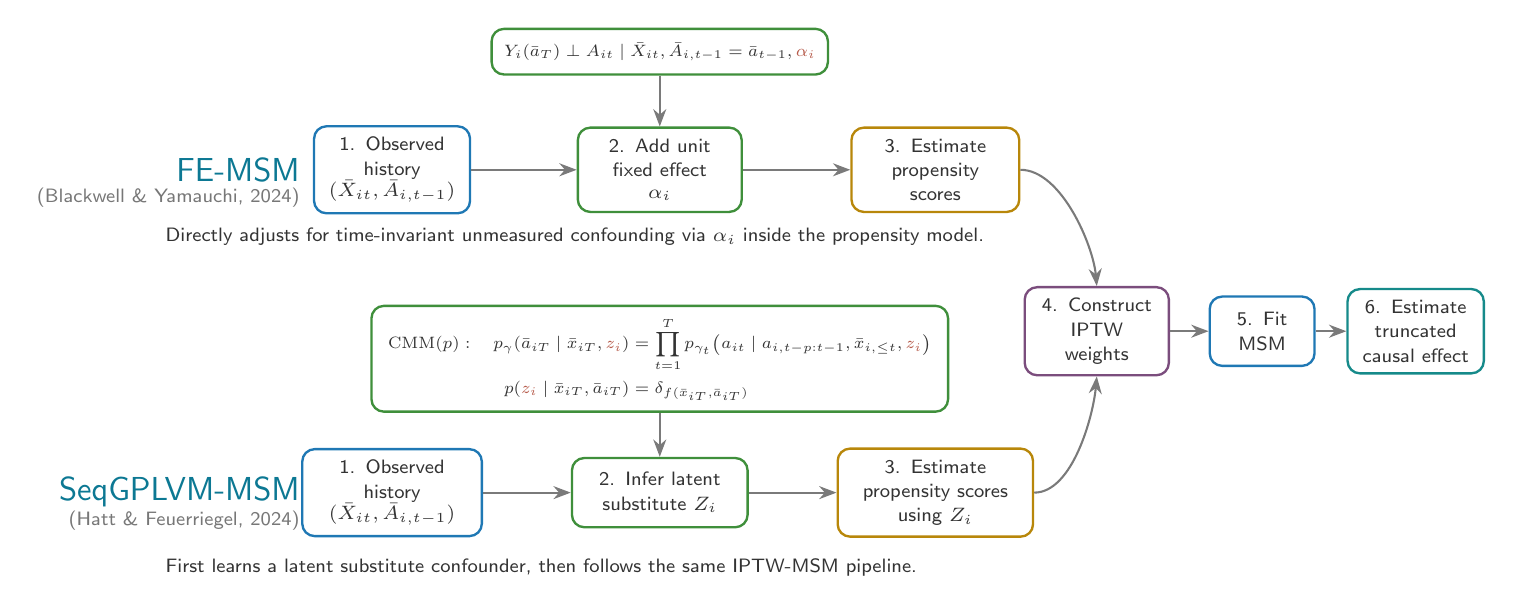
\begin{tikzpicture}[
  x=1cm,y=1cm,
  flow/.style={
    -{Stealth[length=2.2mm]},
    line width=0.75pt,
    draw=PrimerText!65
  },
  stepblue/.style={
    rounded corners=4.5pt,
    line width=0.85pt,
    draw=PipeBlue,
    fill=white,
    align=center,
    minimum height=0.88cm,
    inner sep=4pt,
    font=\fontsize{7.4}{8.8}\selectfont,
    text=PrimerText
  },
  stepgreen/.style={
    rounded corners=4.5pt,
    line width=0.85pt,
    draw=PipeGreen,
    fill=white,
    align=center,
    minimum height=0.88cm,
    inner sep=4pt,
    font=\fontsize{7.4}{8.8}\selectfont,
    text=PrimerText
  },
  stepgold/.style={
    rounded corners=4.5pt,
    line width=0.85pt,
    draw=PipeGold,
    fill=white,
    align=center,
    minimum height=0.88cm,
    inner sep=4pt,
    font=\fontsize{7.4}{8.8}\selectfont,
    text=PrimerText
  },
  steppurple/.style={
    rounded corners=4.5pt,
    line width=0.85pt,
    draw=PipePurple,
    fill=white,
    align=center,
    minimum height=0.92cm,
    inner sep=4pt,
    font=\fontsize{7.4}{8.8}\selectfont,
    text=PrimerText
  },
  stepteal/.style={
    rounded corners=4.5pt,
    line width=0.85pt,
    draw=PipeTeal,
    fill=white,
    align=center,
    minimum height=0.92cm,
    inner sep=4pt,
    font=\fontsize{7.4}{8.8}\selectfont,
    text=PrimerText
  },
  formula/.style={
    rounded corners=4.5pt,
    line width=0.85pt,
    draw=PipeGold,
    fill=white,
    align=center,
    inner sep=4.5pt,
    font=\fontsize{6.7}{8.0}\selectfont,
    text=PrimerText
  },
  methodlabel/.style={
  anchor=east,
  font=\fontsize{12.3}{14.5}\selectfont,
  text=PrimerTeal
  },
  sidenote/.style={
    anchor=west,
    font=\fontsize{7.4}{9.0}\selectfont,
    text=PrimerText,
    align=left
  },
  methodcite/.style={
  anchor=east,
  font=\fontsize{6.8}{8.0}\selectfont,
  text=PrimerMuted
  }
]

% -------------------------------------------------
% Top formula boxes
% -------------------------------------------------
\node[formula, draw=PipeGreen,minimum height=0.58cm] (feassump) at (6.50,5.20)
{\scalebox{0.85}{$
Y_i(\bar a_T)\perp A_{it}
\mid \bar X_{it},\bar A_{i,t-1}=\bar a_{t-1},\red{\alpha_i}
$}};

%\node[formula, minimum height=0.58cm] (femodel) at (10,6.20)
%{\scalebox{0.82}{$
%\operatorname{logit}P(A_{it}=1\mid \bar X_{it},\bar A_{i,t-1},\alpha_i)
%=
%\alpha_i+\beta^\top X_{it}+\phi A_{i,t-1}
%$}};

% -------------------------------------------------
% FE-MSM row
% -------------------------------------------------
\node[methodlabel] at (2.05,3.70) {FE-MSM};
\node[methodcite] at (2.05,3.35) {(Blackwell \& Yamauchi, 2024)};


\node[stepblue, text width=1.70cm] (fe1) at (3.10,3.70)
  {1. Observed\\history\\[-1pt]
  \((\bar X_{it},\bar A_{i,t-1})\)};

\node[stepgreen, text width=1.80cm] (fe2) at (6.50,3.70)
{2. Add unit\\fixed effect\\[-1pt]
\(\alpha_i\)};

\node[stepgold, text width=1.85cm] (fe3) at (10,3.70)
{3. Estimate\\propensity\\scores};

\draw[flow] (fe1.east) -- (fe2.west);
\draw[flow] (fe2.east) -- (fe3.west);
%\draw[flow] (fe3.north)--(femodel.south);
\draw[flow] (feassump.south)--(fe2.north);

\node[sidenote] at (0.10,2.85)
{Directly adjusts for time-invariant unmeasured confounding via \(\alpha_i\) inside the propensity model.};

% -------------------------------------------------
% CMM box
% -------------------------------------------------
\node[
  stepgreen,
  minimum width=6.90cm,
  minimum height=0.82cm,
  inner xsep=6pt,
  inner ysep=4pt
] (cmm) at (6.50,1.30)
{\scalebox{.85}{$
\begin{aligned}
\mathrm{CMM}(p):\quad
p_{\gamma}(\bar a_{iT}\mid \bar x_{iT},\red{z_i})
&=
\prod_{t=1}^{T}
p_{\gamma_t}\!\left(
a_{it}\mid a_{i,t-p:t-1},\bar x_{i,\le t},\red{z_i}
\right)
\\[-1pt]
p(\red{z_i}\mid \bar x_{iT},\bar a_{iT})
&=
\delta_{f(\bar x_{iT},\bar a_{iT})}
\end{aligned}
$}};

% -------------------------------------------------
% SeqGPLVM-MSM row
% -------------------------------------------------
\node[methodlabel] at (2.05,-0.40) {SeqGPLVM-MSM};
\node[methodcite] at (2.05,-0.75) {(Hatt \& Feuerriegel, 2024)};

\node[stepblue, text width=2.00cm] (seq1) at (3.10,-0.40)
{1. Observed\\history\\[-1pt]
\((\bar X_{it},\bar A_{i,t-1})\)};

\node[stepgreen, text width=1.95cm] (seq2) at (6.50,-0.40)
{2. Infer latent\\substitute \(Z_i\)};

\node[stepgold, text width=2.20cm] (seq3) at (10,-0.40)
{3. Estimate\\propensity scores\\using \(Z_i\)};

\draw[flow] (seq1.east) -- (seq2.west);
\draw[flow] (seq2.east) -- (seq3.west);
\draw[flow] (cmm.south) -- (seq2.north);

\node[sidenote] at (0.10,-1.35)
{First learns a latent substitute confounder, then follows the same IPTW-MSM pipeline.};

% -------------------------------------------------
% Shared IPTW-MSM pipeline
% -------------------------------------------------
\node[steppurple, text width=1.55cm] (w) at (12.05,1.65)
{4. Construct\\IPTW weights};

\node[stepblue, text width=1.05cm] (msm) at (14.15,1.65)
{5. Fit\\MSM};

\node[stepteal, text width=1.45cm] (effect) at (16.10,1.65)
{6. Estimate\\truncated\\causal effect};

% FE and Seq paths into shared step
\draw[flow] (fe3.east)  to[out=0,in=95,looseness=0.75] (w.north);
\draw[flow] (seq3.east) to[out=0,in=-95,looseness=0.75] (w.south);

% Shared pipeline
\draw[flow] (w.east) -- (msm.west);
\draw[flow] (msm.east) -- (effect.west);

\end{tikzpicture}%
}
\end{center}

\end{frame}
%%%%%%%%%%%%%%%%%%%%%%%%%%%%%%%%%%%%%%%%%%%%%%%%%%%
\begin{comment}
% Speaker note: 55 seconds. Contrast the two methods without getting lost in detail: fixed effect versus latent variable inferred from the treatment trajectory.
\begin{frame}{Two methods, one IPTW-MSM pipeline}
\begin{columns}[T,onlytextwidth]
\begin{column}{0.46\textwidth}
{\fontsize{11.0}{14}\selectfont\teal{FE-MSM}}\par
\vspace{0.18cm}

\includegraphics[width=0.74\linewidth]{fixed_effect_dag.pdf}
\vspace{0.08cm}
\spacedparagraph{Use a unit fixed effect \(\alpha_i\) directly in the propensity model.}
\[
\eta_i=\alpha_i
\]
\end{column}
\begin{column}{0.50\textwidth}
{\fontsize{11.0}{14}\selectfont\teal{SeqGPLVM-MSM}}\par
\vspace{0.18cm}

\includegraphics[width=0.92\linewidth]{fit_seqgplvm_dag.pdf}
\vspace{-0.05cm}
\spacedparagraph{Infer a latent variable \(Z_i\) from the treatment trajectory and covariates.}
\[
\eta_i=Z_i
\]
\end{column}
\end{columns}
\vspace{0.10cm}
{\fontsize{9.7}{12.5}\selectfont\RaggedRight Both methods 
then estimate propensity scores, construct IPTW weights, 
and fit the same truncated marginal structural model.\par}
\end{frame}
\end{comment}
% Speaker note: 50 seconds. Explain why the simulation is fair: known DGP, true effects known, same MSM, same target. Stress this uses the final thesis design, not the older draft results.


% Speaker note: 65 seconds. This is the most important slide. Summarize results accurately from the thesis: both methods help versus naive IPTW, FE-MSM usually better, SeqGPLVM weak with short T/strong U, coverage mixed.
\begin{frame}{Results: adjustment helps, but finite samples matter}
\begin{columns}[T,onlytextwidth]
\begin{column}{0.54\textwidth}
\vspace{0.0cm}
\includegraphics[width=0.96\linewidth]{results_a2.png}
\end{column}
\begin{column}{0.42\textwidth}
\vspace{0.05cm}
{\fontsize{8.7}{11.3}\selectfont
\spacedparagraph{Naive IPTW stays biased when \(U_i\) is ignored.}
\spacedparagraph{Both methods \teal{reduce bias}, especially with longer treatment histories.}
\spacedparagraph{FE-MSM has \teal{lower bias and standard error} in this DGP.}
\spacedparagraph{SeqGPLVM-MSM is most fragile for \(\rho=50\), especially under stronger unmeasured confounding.}
\arrowtext{Coverage is mixed; neither method is an automatic fix.}
}
\end{column}
\end{columns}
\smallref{Shown: two-covariate case with stronger unmeasured confounding, \(a=2\); 500 simulation runs.}
\end{frame}

% Speaker note: 55 seconds. End with a balanced conclusion: the thesis is not just a benchmark, it clarifies assumptions and shows what is needed before practical use.
\begin{frame}{Conclusion: what the comparison shows}
\begin{columns}[T,onlytextwidth]
\begin{column}{0.48\textwidth}
{\fontsize{11}{14}\selectfont\teal{Main contributions}}\par
\vspace{0.25cm}
\spacedparagraph{Unified notation and assumptions for FE-MSM and SeqGPLVM-MSM.}
\spacedparagraph{A detailed derivation of the SeqGPLVM loss function and a modular GPyTorch implementation.}
\spacedparagraph{A simulation comparison under a common causal target and DGP.}
\end{column}
\begin{column}{0.48\textwidth}
{\fontsize{11}{14}\selectfont\teal{Main takeaway}}\par
\vspace{0.25cm}
\spacedparagraph{Both methods replace the usual no-unmeasured-confounding assumption with structural assumptions about a time-invariant hidden factor.}
\spacedparagraph{FE-MSM is simpler and more stable here, but depends on correct propensity specification and within-unit switching.}
\spacedparagraph{SeqGPLVM is more flexible, but relies on strong latent-identifiability assumptions and enough treatment history.}
\end{column}
\end{columns}
\vspace{0.25cm}
{\fontsize{10.3}{14}\selectfont\RaggedRight\red{Bottom line:} promising tools in controlled settings, but not yet general-purpose deconfounding methods.\par}
\end{frame}

\end{document}
